\documentclass{beamer}
\usepackage[utf8]{inputenc}
\usepackage{caption}
\usetheme{Madrid}
\usecolortheme{default}

%------------------------------------------------------------
%This block of code defines the information to appear in the
%Title page
\title[Analysing Urban form using big data] %optional
{Analysing Urban form using big data}

\subtitle{A primer for urban data science in python}

\author[Christina, Last] % (optional)
{C.~K.~Last}

\institute[ATI] % (optional)
{
  The Alan Turing Institute\\
  The UK's Institute for Artificial Intelligence and Data Science
}

\date[CUS 2021] % (optional)
{Center for Urban Studies, Kyiv National University, October 2021}

%End of title page configuration block
%------------------------------------------------------------



%------------------------------------------------------------
%The next block of commands puts the table of contents at the
%beginning of each section and highlights the current section:

\AtBeginSection[]
{
  \begin{frame}
    \frametitle{Table of Contents}
    \tableofcontents[currentsection]
  \end{frame}
}
%------------------------------------------------------------


\begin{document}

%The next statement creates the title page.
\frame{\titlepage}


%---------------------------------------------------------
%This block of code is for the table of contents after
%the title page
\begin{frame}
\frametitle{Table of Contents}
\tableofcontents
\end{frame}
%---------------------------------------------------------


\section{Background}

%---------------------------------------------------------
%Changing visivility of the text
\begin{frame}
\frametitle{Background}
I am Christina Last, and I use data to understand our built environment.
\begin{itemize}
    \item<1-> BSc Geography at the University of Bristol, UK
    \item<2-> Worked in New York on largest US urban plans
    \item<3-> Lectured at Harvard
    \item<4-> Lead Data Scientist at property technology startup
    \item<5-> Tech Lead at UNICEF
    \item<6-> Researcher at Alan Turing Institute
\end{itemize}
\end{frame}

%---------------------------------------------------------

\section{Urban Form}

%---------------------------------------------------------
\begin{frame}{Urban Form}
\begin{figure}
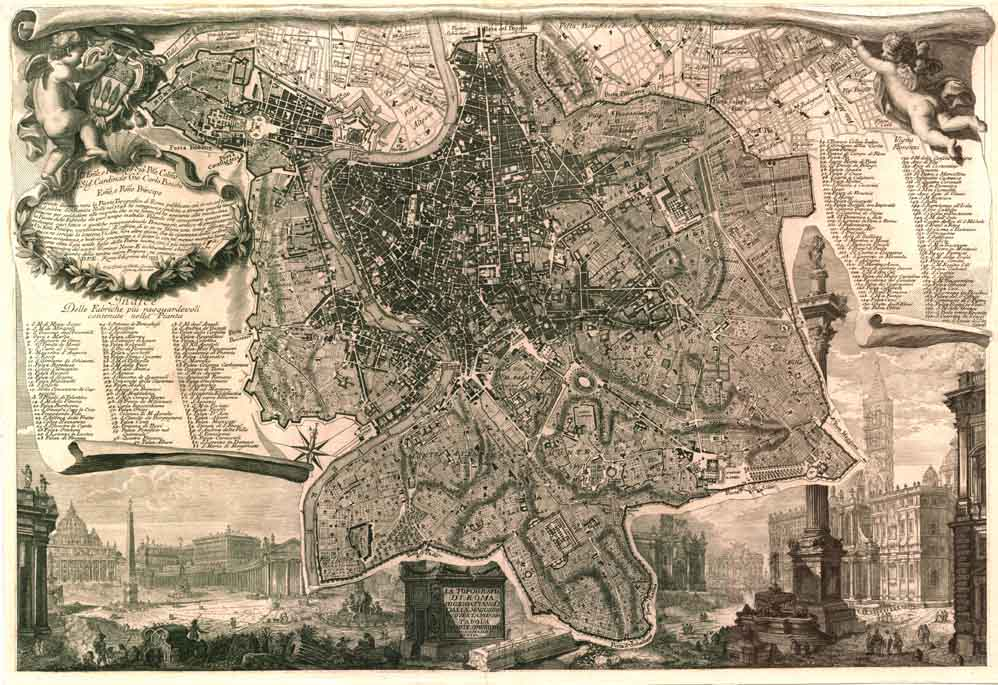
\includegraphics[width=0.8\textwidth]{images/nolli_map_rome.jpg}
\caption{The Nolli map, 1748,  \href{https://commons.wikimedia.org/wiki/File:Nolli_map1.jpg}{wikipedia}}
\end{figure}
\end{frame}

%---------------------------------------------------------

\begin{frame}{Urban Form}
\begin{figure}
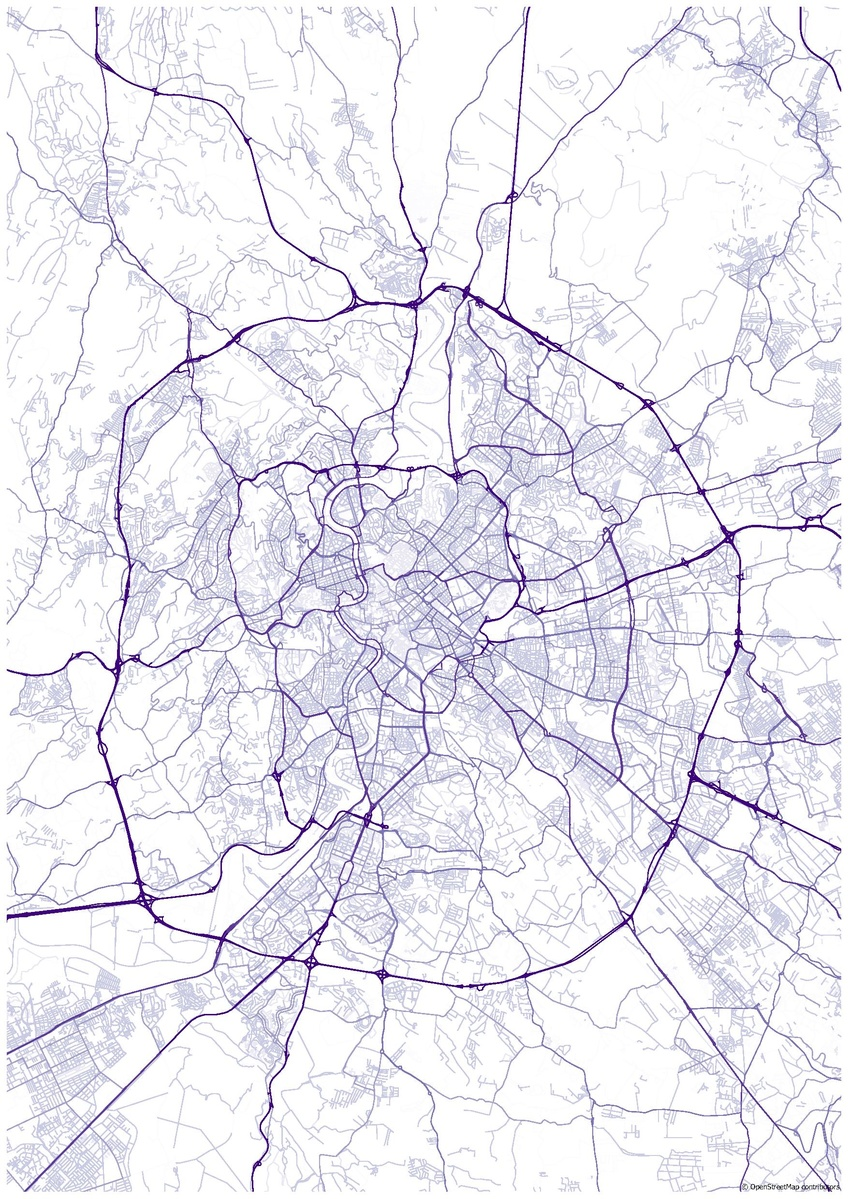
\includegraphics[height=0.5\textwidth]{images/osm_map_rome.jpg}
\caption{Map of Rome created for the State of the Map 2019 social event by Adam Rousell and Sabrina Marx using OpenStreetMap data and QGIS.}
\end{figure}
\end{frame}


%---------------------------------------------------------

\begin{frame}{Urban Form}
\begin{figure}
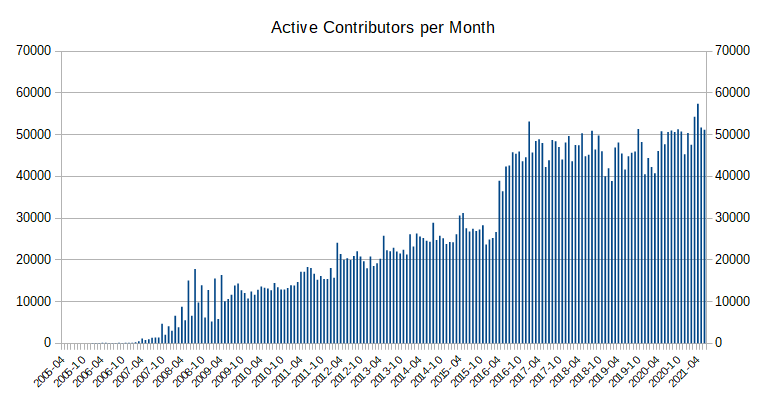
\includegraphics[height=0.5\textwidth]{images/osm_contributors_month.png}
\caption{Contributions to open source mapping has been growing, \href{https://blog.openstreetmap.org/2021/02/25/100-million-edits-to-openstreetmap/}{reaching 100 million contributions this year}}
\end{figure}
\end{frame}

%---------------------------------------------------------
%Example of the \pause command
\begin{frame}
In the age of ubiquitous urban data \pause

computational toolkits open up a new era of worldwide
urban form analysis \pause

to integrated quantitative and qualitative perspectives into urban planning.
\end{frame}
%---------------------------------------------------------

\section{Python for urban data science}

%---------------------------------------------------------
%Highlighting text
\begin{frame}
\frametitle{Python for urban data science}

Spatial information (and in turn information management) plays a central role in urban planning as nearly all urban and human processes are spatially-situated. \pause


User-contributed big data about spatial infrastructure that allow us to examine the physical flows of people, goods, and information through urban space.

\end{frame}

%---------------------------------------------------------
%Two columns
\begin{frame}{Python for urban data science}
\begin{figure}

\begin{columns}[t]

\column{.5\textwidth}
\centering

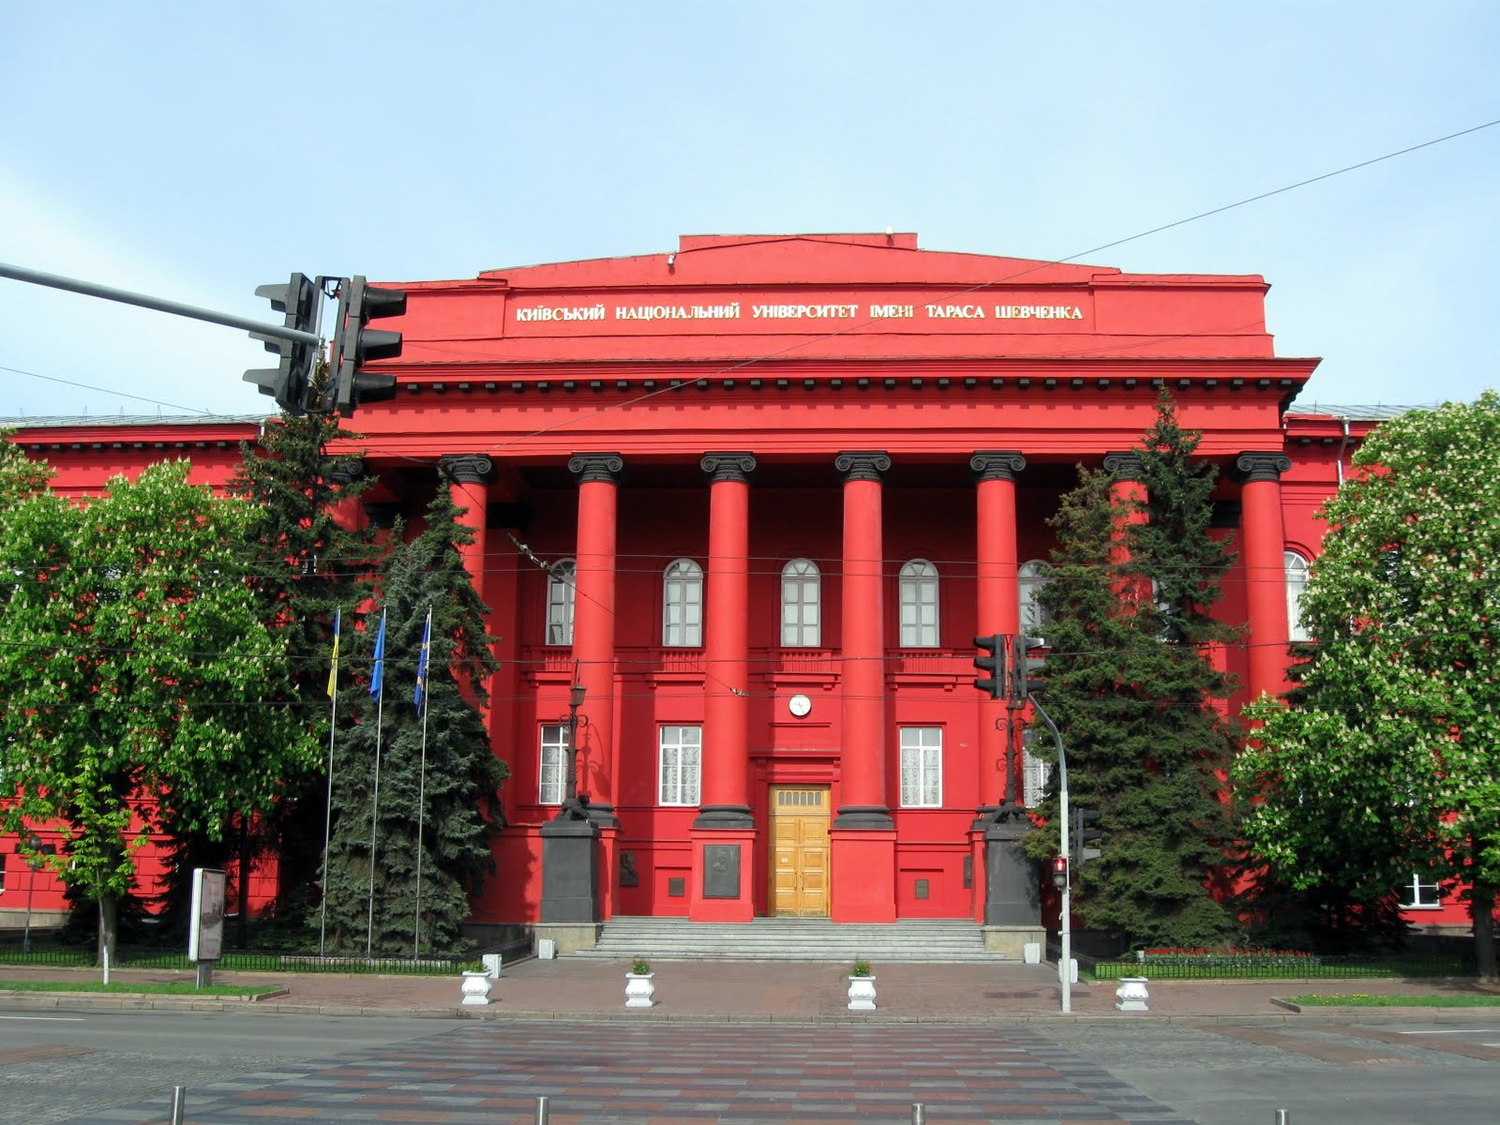
\includegraphics[width=3cm,height=3cm]{images/point_kyiv.jpg}
\captionof{figure}{Kyiv}
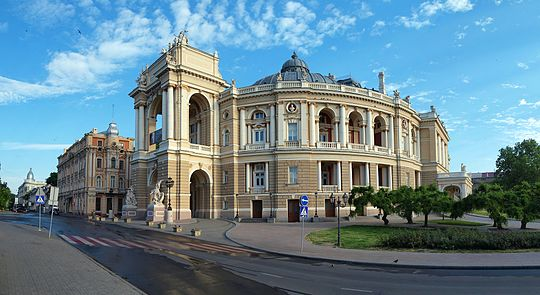
\includegraphics[height=3cm]{images/point_odesa.jpg}
\captionof{figure}{Odesa}
\column{.5\textwidth}
\begin{center}

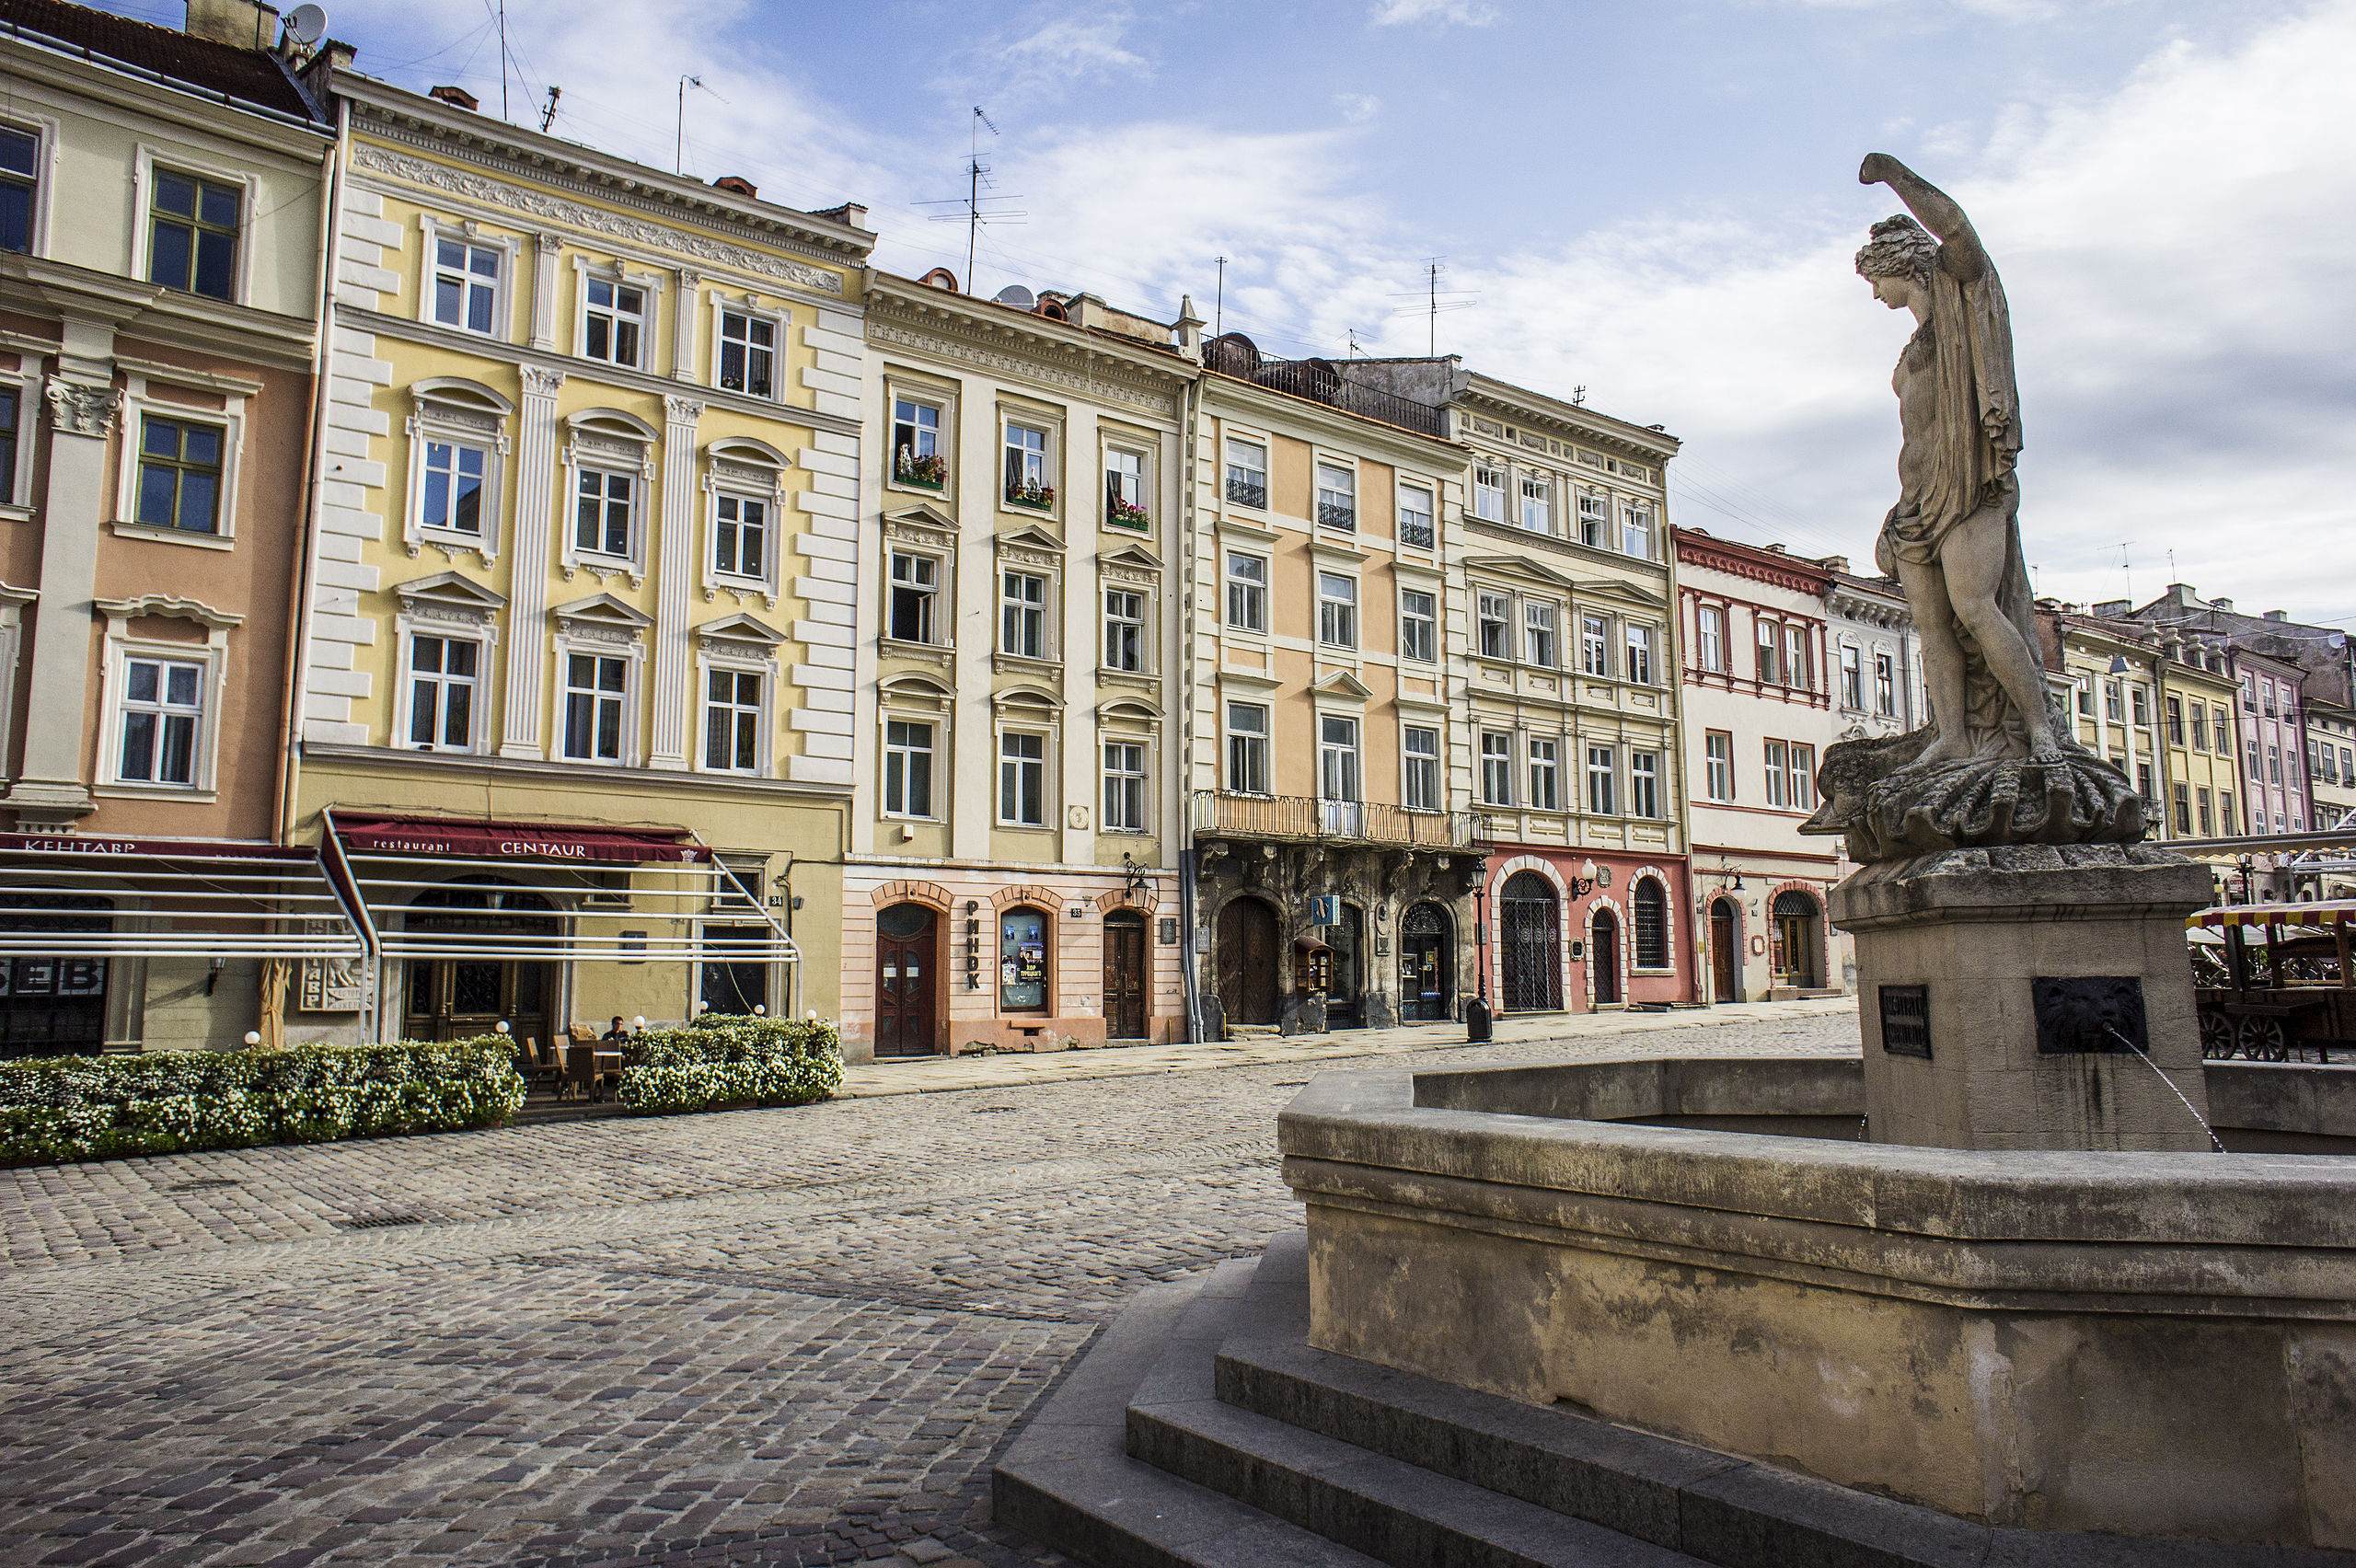
\includegraphics[height=3cm]{images/point_lviv.jpg}
\captionof{figure}{Lviv}
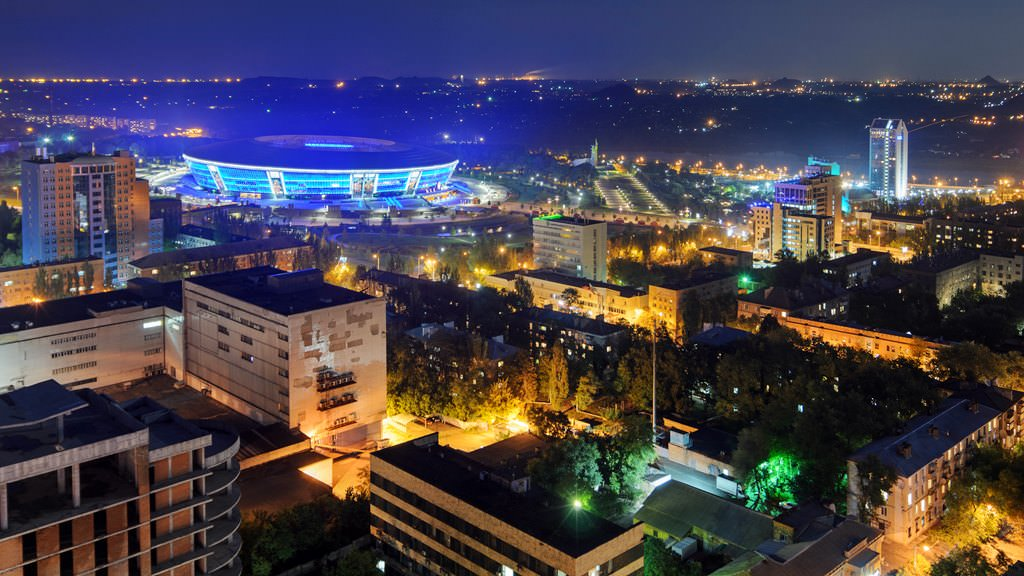
\includegraphics[height=3cm]{images/point_donetsk.jpg}
\captionof{figure}{Donetsk}
\end{center}

\end{columns}
\end{figure}
\end{frame}

%---------------------------------------------------------
%Two columns
\begin{frame}{Python for urban data science}
\begin{figure}

\begin{columns}[t]

\column{.5\textwidth}
\centering

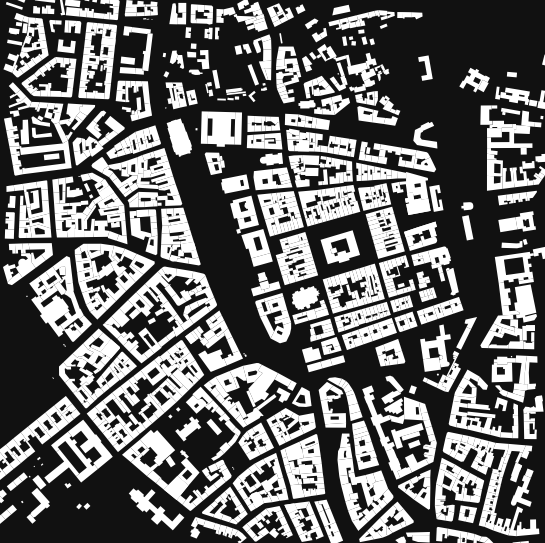
\includegraphics[width=3cm,height=3cm]{images/Kyiv1km_bldgs.png}
\captionof{figure}{Kyiv}
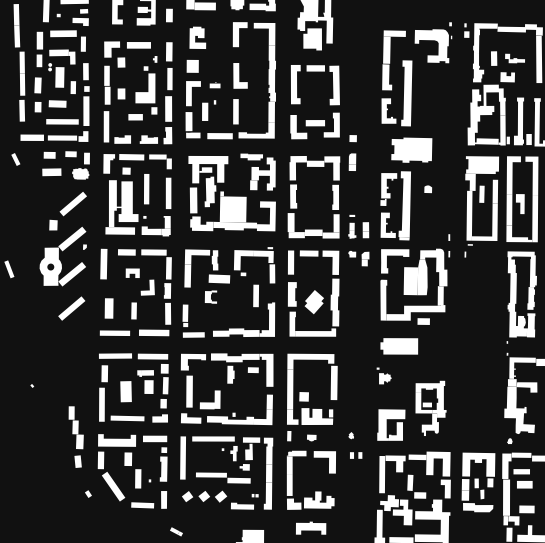
\includegraphics[width=3cm,height=3cm]{images/Odesa1km_bldgs.png}
\captionof{figure}{Odesa}
\column{.5\textwidth}
\begin{center}

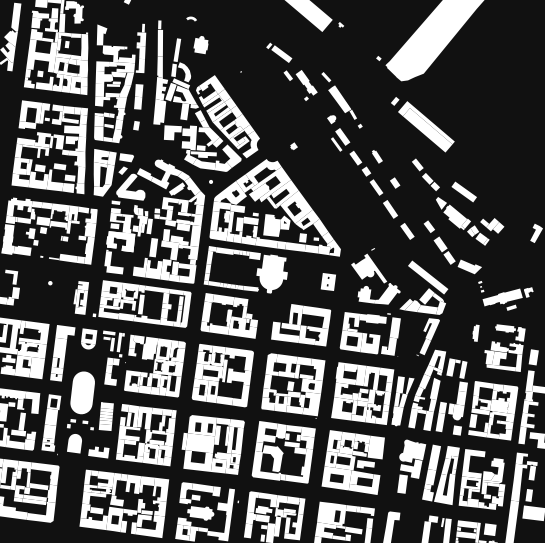
\includegraphics[width=3cm,height=3cm]{images/Lviv1km_bldgs.png}
\captionof{figure}{Lviv}

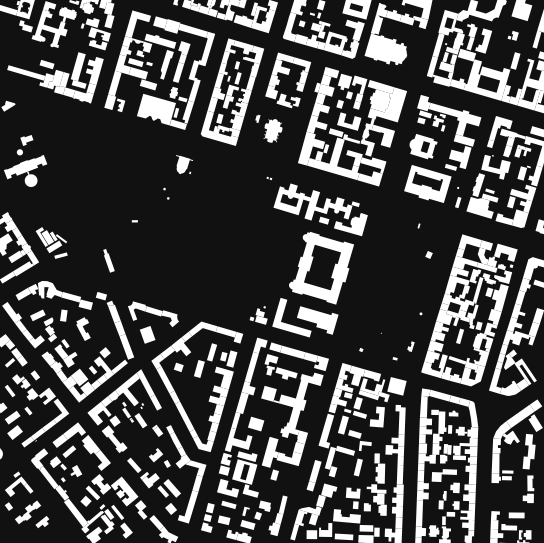
\includegraphics[height=3cm]{images/Donetsk1km_bldgs.png}
\captionof{figure}{Donetsk}
\end{center}

\end{columns}
\end{figure}
\end{frame}

%---------------------------------------------------------
%Two columns
\begin{frame}{Python for urban data science}
\begin{figure}

\begin{columns}[t]

\column{.5\textwidth}
\centering

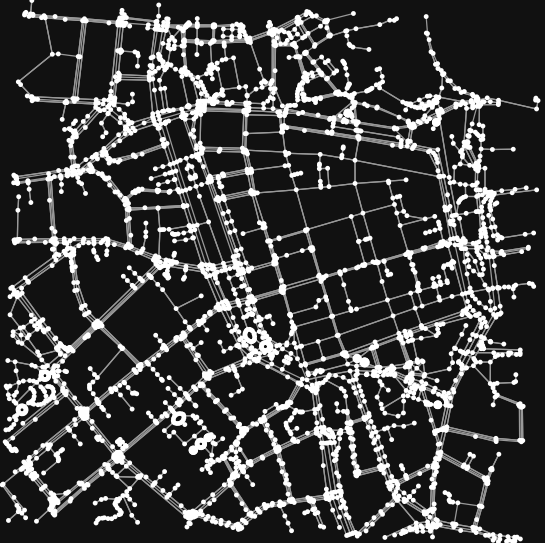
\includegraphics[width=3cm,height=3cm]{images/Kyiv1km_streets.png}
\captionof{figure}{Kyiv}
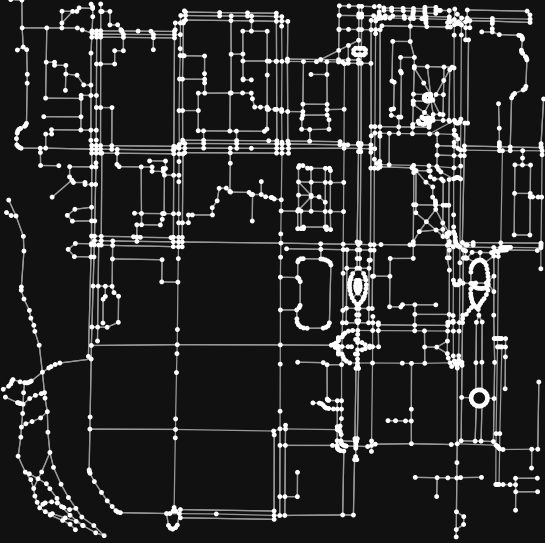
\includegraphics[width=3cm,height=3cm]{images/Odesa1km_streets.png}
\captionof{figure}{Odesa}
\column{.5\textwidth}
\begin{center}

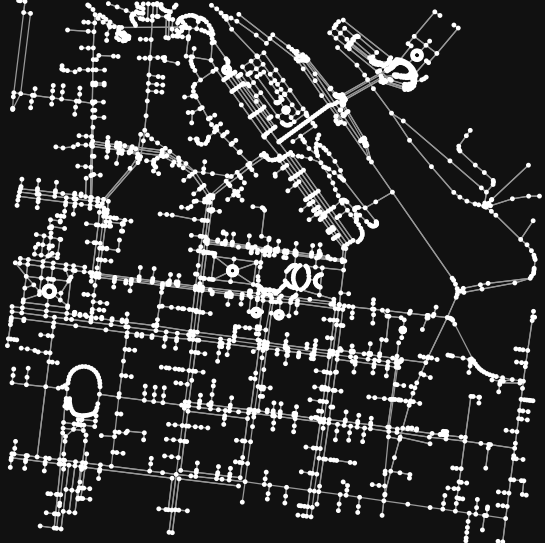
\includegraphics[width=3cm,height=3cm]{images/Lviv1km_streets.png}
\captionof{figure}{Lviv}

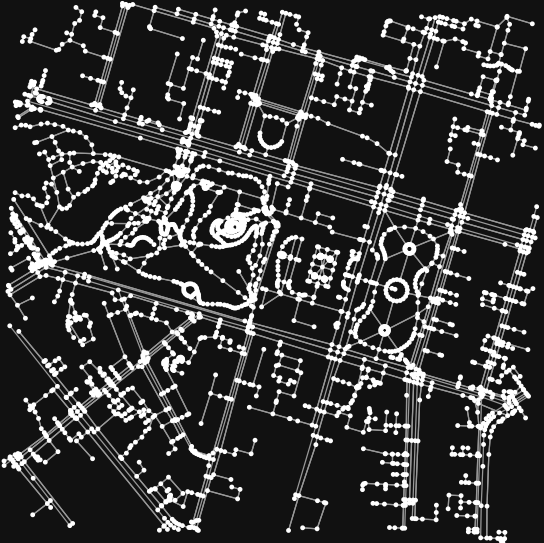
\includegraphics[height=3cm]{images/Donetsk1km_streets.png}
\captionof{figure}{Donetsk}
\end{center}

\end{columns}
\end{figure}
\end{frame}

%---------------------------------------------------------
\begin{frame}{Python for urban data science}
\begin{figure}
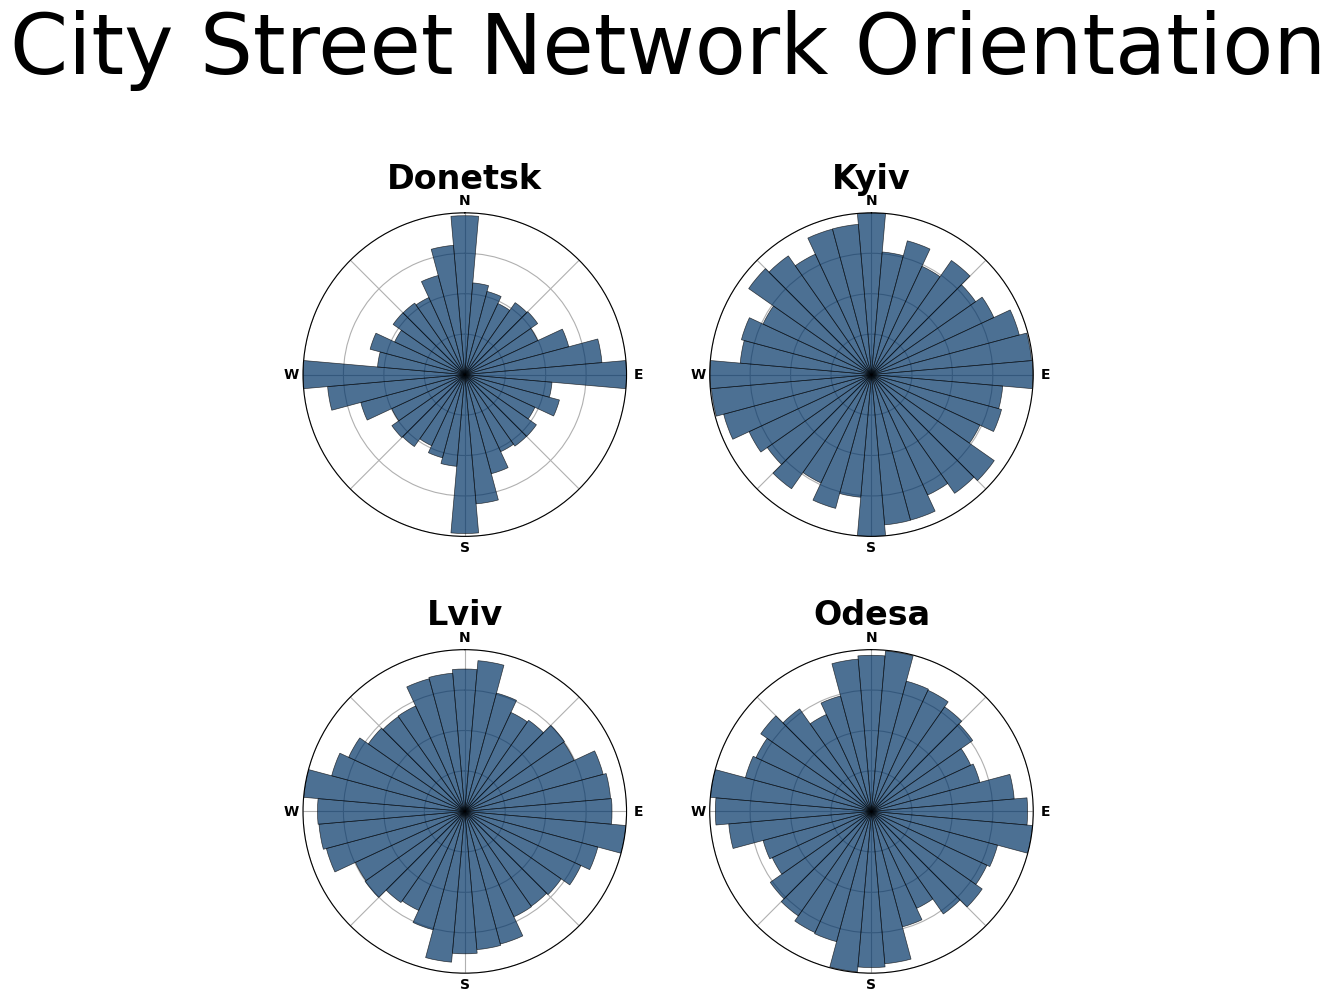
\includegraphics[width=0.8\textwidth]{images/street-orientations.png}
\caption{Rose diagrams of the street orientations in Ukraine's major cities}
\end{figure}
\end{frame}


%---------------------------------------------------------
%Example of the \pause command
\begin{frame}
Through the tools of urban morphology and computer science, spatial information allows us  to see how urban planning, design organize and order space \cite{Boeing2017}.  \pause

Today, OSM provides user-generated big data to perform
these urban data science workflows automatically. \pause

The rose diagrams compress the complexity of street network orientation to help us understand similarities and differences in the spatial ordering of the city’s streets \cite{Boeing2019}.
\end{frame}
%---------------------------------------------------------
\begin{frame}
\frametitle{References}
\bibliographystyle{amsalpha}
\bibliography{references.bib}
\end{frame}
%------------------------------------------------------------
%------------------------------------------------------------

\end{document}
